\documentclass[expanded]{lkx_pset}

\title{CS181 Problem Set 1}
\author{Lev Kruglyak}
\due{February 10, 2024}

\usepackage{pgfplots}
\pgfplotsset{compat=1.14}
\usepackage[outputdir=build]{minted}
\usepackage{graphicx}


\collaborator{AJ LaMotta}

\begin{document}
\maketitle

\begin{problem}{1}[Setting up the Regression]
Your goal is to predict temperature variation given the year.  Before we start deriving and coding up our regressions, we will interrogate the set-up of our problem.
\end{problem}

\begin{parts}
	\begin{part}{a}
		These data were derived from ice core samples in Antarctica.
		Take a brief look at the
		\href{https://www.ncei.noaa.gov/pub/data/paleo/icecore/antarctica/epica_domec/edc3deuttemp2007.txt}{original
			data file}. Briefly discuss how the data were processed: what kinds of
		decisions and corrections had to be made?  We know that different
		places on earth have different temperatures: what does the
		temperature in the temperature column correspond to?
	\end{part}

	Reading the source, we can see that several corrections were made. For example, temperatures were corrected for sea-water isotropic composition and for ice sheet elevation. Also, temperatures are not recorded on an absolute scale but as a change in temperature from a rolling average of previous changes.

	\begin{part}{b}
		Even before doing any formal regressions, we see that there is
		some periodicity in the data: there are years that are warmer, and
		years that are cooler.  Suppose you are a government official
		advising on how much to worry about climate change.  Would it be
		reasonable to use this pattern as evidence that the earth will
		cool down again?  Why or why not, or to what extent?
	\end{part}

	While there does appear to be some peridocity, using the dataset to predict anything too far into the future would be tricky, since temperature variation is an incredibly complex system with lots of factors. For example, volcanic erruptions or human CO2 emissions could alter the temperature on small timeframes, breaking any pattern deduced by the regression.

	\begin{part}{c}
		In the problems below, we will focus on interpolating
		temperatures for years not provided in the training set.  What
		kind of application would such a regression be useful for?
	\end{part}

	The main application would be predicting future temperature variations, or making estimates of temperature variations so long ago that measuring directly would be infeasible.
\end{parts}

\begin{problem}{2}[Optimizing a Kernel]
Kernel-based regression techniques are similar to nearest-neighbor
regressors: rather than fit a parametric model, they predict values
for new data points by interpolating values from existing points in
the training set.  In this problem, we will consider a kernel-based
regressor of the form:
\begin{equation*}
	f_\tau(x^*) = \cfrac{\sum_{n} K_\tau(x_n,x^*) y_n}{\sum_n K_\tau(x_n, x^*)}
\end{equation*}
where $\mathcal{D}_\texttt{train} = \{(x_n,y_n)\}_{n = 1} ^N$ are the
training data points, and $x^*$ is the point for which you want to
make the prediction.  The kernel $K_\tau(x,x')$ is a function that
defines the similarity between two inputs $x$ and $x'$. A popular
choice of kernel is a function that decays as the distance between the
two points increases, such as
\begin{equation*}
	K_\tau(x,x') = \exp\left\{-\frac{(x-x')^2}{\tau}\right\}
\end{equation*}
where $\tau$ represents the square of the lengthscale (a scalar value that
dictates how quickly the kernel decays).  In this
problem, we will consider optimizing what that (squared) lengthscale
should be.
\end{problem}

\begin{parts}
	\begin{part}{a}
		Let's first take a look at the behavior of the fitted model for different values of $\tau$. Implement the \texttt{kernel\_regressor} function in the notebook, and plot your model for years in the range $800,000$ BC to $400,000$ BC at $1000$ year intervals for the following three values of $\tau$: $1, 50, 2500$.
		Since we're working in terms of thousands of years, this means you should plot $(x, f_\tau(x))$ for $x = 400, 401, \dots, 800$. Describe how the fits change with $\tau$.
	\end{part}

	\begin{figure}[ht]
		\centering
		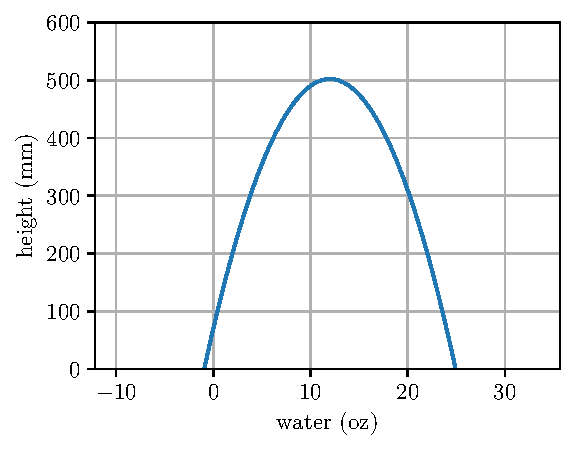
\includegraphics[]{build/2a.pdf}
	\end{figure}\noindent
	As we can see, as $\tau$ decreases, the curve fits the training data points closer and closer. As $\tau$ increases, the curve generalizes more, is smoother, and shows the general trends of the data.

	\begin{part}{b}
		Now, we will evaluate the quality of each model \emph{quantitatively} by computing the error on some test set $\mathcal{D}_\texttt{test} = \{(x'_m, y'_m)\}_{m = 1} ^M$.  Write down the expression for MSE of $f_\tau$ over the test set as a function of the training set and test set. Your answer may include $\{(x'_m, y'_m)\}_{m = 1} ^M$, $\{(x_n, y_n)\}_{n = 1} ^N$, and $K_\tau$, but not $f_\tau$.
	\end{part}

	Using the mean squared error formula and the definition for our estimator, we can write
	\[
		\mathrm{MSE} = \frac{1}{M} \sum_{1\leq m \leq M} \left(y'_m - f_\tau(x'_m)\right)^2
		= \frac{1}{M}\sum_{1\leq m \leq M} \left(y'_m - \frac{\sum_{n=1}^N K_\tau(x_n, x'_m)y_n}{\sum_{n=1}^N K_\tau(x_n, x'_m)}\right)^2.
	\]

	\begin{part}{c}
		Suppose we used the training set as our test set, that is, we evaluated the expression above with $\mathcal{D}_\texttt{test} = \mathcal{D}_\texttt{train}$, and chose the value of $\tau$ which gave the smallest loss.  What value of $\tau$ would be picked?  Why is setting $\mathcal{D}_\texttt{test} = \mathcal{D}_\texttt{train}$ a bad idea?
	\end{part}

	Suppose we set $\mathcal{D}_{\texttt{test}}=\mathcal{D}_{\texttt{train}}$, then the expression for $\mathrm{MSE}$ is
	\[
		\mathrm{MSE} = \frac{1}{N}\sum_{1\leq m \leq N} \left(y_m - \frac{\sum^N_{n=1} K_\tau(x_n, x'_m)y_n}{\sum^N_{n=1} K_\tau(x_n, x'_m)}\right).
	\]
	Notice that as $\tau \to 0$, we have the convergence $K_\tau(x, x^*)\to \mathbb{I}_{\{x\}}(x^*)$ of the kernel function to an indicator variable. This means that $f_\tau(x^*)$ converges to the step function
	\[
		\widetilde{f}_\tau(x^*) = y_{i(x^*)}\quad\textrm{where}\quad i(x^*)=\mathrm{argmin}_{1\leq n \leq N} |x^* - x_n|.
	\]
	In particular, for any $(x,y)\in \mathcal{D}_\texttt{test}$ we have $\widetilde{f}_\tau(x)=y$. In other words, the estimator is perfect on the ``test'' dataset in the limit as $\tau \to 0$. The optimal $\tau$ then must be extremely small. (A value of $\tau=0$ is impossible, unless the expressions in the definition of the estimator are replaced with their limit as $\tau = 0$.)

	This is clearly not very useful -- our model has completely overfit the data and became a $k$-means clustering estimator with $k=1$, losing the beneficial features of the kernel estimator.

	% \emph{Hint: consider what value of $\tau$ would be optimal, for $\tau$ ranging in $(0, \infty)$. We can consider $f_\tau(x^*)$ as a weighted average of the training responses, where the weights are proportional to the distance to $x^*$, and the distance is computed via the kernel. What happens to $K_\tau(x, x')$ as $\tau$ becomes very small, when $x = x'$? What about when $x \neq x'$?}

	\begin{part}{d}
		Let us compute the MSE on the provided test set (that is, not the training set). Write Python code to compute the MSE with respect to the same lengthscales as in (a). Which model yields the lowest test set MSE?
	\end{part}

	Calculating the MSE for the data we plotted in (a), we obtain the following data:
	\begin{center}
		\renewcommand*{\arraystretch}{1.2}
		\begin{tabular}{|c|c|}
			\hline
			$\tau$ & $\textrm{MSE}$ \\
			\hline
			1      & 1.947          \\
			50     & 1.858          \\
			2500   & 8.334          \\
			\hline
		\end{tabular}
	\end{center}
	We can see that the model with $\tau = 50$ yields the lowest error. This makes sense if we look at the graph in (a) -- when $\tau$ is very low, the model overfits to the points in the training data set and might deviate too much from the points in the test data set.

	\begin{part}{e}
		Describe the time and space complexity of kernelized regression with respect to the size of the training set $N$.
		How, if at all, does the size of the model---everything that needs to be stored to make predictions---change with the size of the training set $N$?
		How, if at all, do the number of computations required to make a prediction for some input $x^*$ change with the size of the training set $N$?
	\end{part}

	There are a variety of optimizations we could make to improve space and time complexity, however for the purposes of this problem let's assume no optimizations were made. For storage, we need to store the entire training dataset, or $2N$ numbers. This means storage complexity is $O(N)$. Similarly, assuming the kernel is constant time to evaluate, the time complexity to perform an estimation is $O(N)$. Thus, both factors scale linearly with the size of the training set.
\end{parts}

\begin{problem}{3}[Kernels and kNN]
Now, let us compare the kernel-based approach to an approach based on
nearest-neighbors.  Recall that kNN uses a predictor of the form
\begin{equation*}
	f(x^*) = \frac{1}{k} \sum_n y_n \mathbb{I}(x_n \texttt{ is one of k-closest to } x^*)
\end{equation*}

\noindent where $\mathbb{I}$ is an indicator variable. For this problem, you will use the \textbf{same dataset as in Problem 1}. Write your own tests!
\end{problem}

\begin{parts}
	\begin{part}{a}
		The kNN implementation \textbf{has been provided for you} in the notebook. Run the cells to plot the results for $k=\{1, 3, N-1\}$, where $N$ is the size of the dataset.

		Describe what you see: what is the behavior of the functions in
		these three plots?  How does it compare to the behavior of the
		functions in the three plots from Problem 1? In particular, are
		there situations in which kNN and kernel-based regression
		interpolate similarly?
	\end{part}

	\begin{figure}[ht]
		\centering
		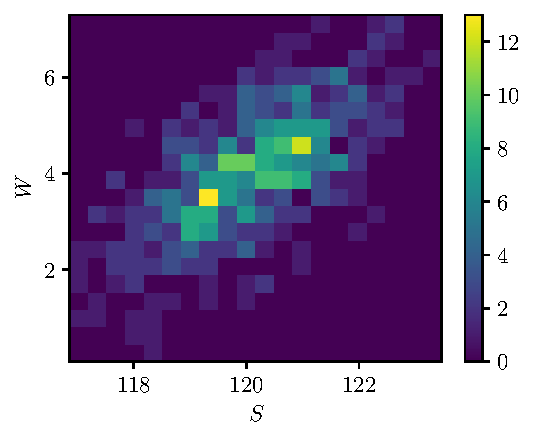
\includegraphics[]{build/3a.pdf}
	\end{figure}\noindent

	The behavior of the $k$-means clustering estimator is quite similar to the behavior of the kernel estimator, however the kernel estimator is smoother. The observations about increasing/decreasing $\tau$ in the kernel estimator correspond to increasing/decreasing $k$.

	\begin{part}{b}
		Compute the MSE on the test set for each value of $k$.  Which solution has the lowest MSE?
	\end{part}

	Doing the same calculations as before, we see that the best model has $k=1$.
	\begin{center}
		\renewcommand*{\arraystretch}{1.2}
		\begin{tabular}{|c|c|}
			\hline
			$k$ & $\textrm{MSE}$ \\
			\hline
			1   & 1.741          \\
			3   & 3.891          \\
			56  & 9.529          \\
			\hline
		\end{tabular}
	\end{center}

	\begin{part}{c}
		As in Problem 1, describe the space and time complexity of kNN.  How does what is stored to compute predictions change with the size of the training set $N$?  How does the computation needed to compute the prediction for a new input depend on the size of the training set $N$? (For the latter, justify based off of your implementation.)
	\end{part}

	As before, the space complexity is $O(N)$ since we need to store all of the training data. The time complexity is also $O(N)$ since finding the $k$-nearest neighbors requires searching all points in the dataset and finding the $k$ smallest elements. We could also account for the space and time complexity of storing and sorting the $k$ smallest elements, however this is independent of $N$ assuming $k$ is. In particular, note that we don't have to sort the entire array of $N$ data points to get the $k$ smallest elements -- rather we can keep some data structure of size complexity $O(k)$ and insert values into it with time complexity $O(k)$ for each iteration through the training data set.
\end{parts}

\begin{problem}{4}[Modeling Climate Change 800,000 Years Ago]
Our last regression will be linear regression.  We currently only have
a one dimensional input, the year.  To create a more expressive linear
model, we will introduce basis functions.
\end{problem}

\begin{parts}
	\begin{part}{a}
		We will first implement the four basis regressions below. Note that we introduce an addition transform $f$ to address concerns about numerical instabilities.
		\begin{enumerate}[(a)]
			\item $\phi_j(x)= f(x)^j$ for $j=1,\ldots, 9$. $f(x) = \frac{x}{1.81 \cdot 10^{2}}.$
			\item $\phi_j(x) = \exp\left\{-(f(x)-\mu_j)^2/5\right\}$ for $\mu_j=\frac{j + 7}{8}$ with $j=1,\ldots, 9$. $f(x) = \frac{x}{4.00 \cdot 10^{2}}.$
			\item $\phi_j(x) =  \cos(f(x) / j)$ for $j=1, \ldots, 9$. $f(x) = \frac{x}{1.81}$.
			\item $\phi_j(x) = \cos(f(x) / j)$ for $j=1, \ldots, 49$. $f(x) = \frac{x}{1.81 \cdot 10^{-1}}$.
		\end{enumerate}

		For each basis create a plot of your code graphing the least squares regression line trained on your training data against a scatter plot of the training data. Boilerplate plotting code is provided in the notebook.
	\end{part}

	Using the standard equations for linear regression with basis functions, we get the following graphs:
	\begin{figure}[ht]
		\centering
		\includegraphics[]{build/4a.pdf}
	\end{figure}\noindent

	\begin{part}{b}
		Now we have trained each of our basis regressions.  For each basis
		regression, compute the MSE on the test set.  Discuss: do any of the
		bases seem to overfit?  Underfit?  Why?
	\end{part}
	Computing the MSE (for both training and testing data) gives us the following table:

	\begin{center}
		\renewcommand*{\arraystretch}{1.2}
		\begin{tabular}{|c|c|c|}
			\hline
			basis function & $\textrm{MSE}_\textrm{test}$ & $\textrm{MSE}_\textrm{train}$ \\
			\hline
			(a)            & 7.956                        & 4.825                         \\
			(b)            & 8.708                        & 5.530                         \\
			(c)            & 5.967                        & 2.879                         \\
			(d)            & 58.912                       & 0.643                         \\
			\hline
		\end{tabular}
	\end{center}

	As we can confirm from the plots in the previous part, the basis function (c) has the lowest error on the testing data. Looking at the training MSE as well, we see that (d) overfits the most by far, whereas (a) and (b) underfit. (c) lies at a perfect balance between both metrics.

	\begin{part}{c}
		Briefly describe what purpose the transforms $f$ serve: why are they helpful?
	\end{part}

	The transforms help fight numeric instability present due to the limitations of floating point numbers.
	% Basis functions allow us to introduce nonlinearity into the model, which allows for the modelling of a much more diverse set of problems. Unlike simple linear regression in one dimension, basis functions allow us to introduce significantly more dimensionaltiy to our modelling problem, which allows for a closer fit in many cases.

	\begin{part}{d}
		As in Problems 1 and 2, describe the space and time complexity of linear regression.  How does what is stored to compute predictions change with the size of the training set $N$?  How does the computation needed to compute the prediction for a new input depend on the size of the training set $N$?  How do these complexities compare to those of the kNN and kernelized regressor?
	\end{part}

	For a linear regression with basis functions, both the storage and time complexity are $O(1)$, since we only need to store the constant size weight matrix, unlike the previous two estimators which required us to store the whole dataset. This makes linear regression much more efficient, however it might not be as accurate for dataset with exceptionally complex features.

	\begin{part}{e}
		Briefly compare and contrast the different regressors: kNN,
		kernelized regression, and linear regression (with bases).  Are some
		regressions clearly worse than others?  Is there one best
		regression?  How would you use the fact that you have these multiple
		regression functions?
	\end{part}

	I think as with many such problems, it depends on the dataset. If the dataset follows a simple linear or polynomial, or even periodic distribution, linear regression will be able to very efficiently extrapolate a pattern, and generalize it quite well. This would also take up much less space that the other two regressors, and be more efficient in calculation. On the other hand, if we have some very unpredictable dataset such as a stock valuation history, a kNN or kernelized regression might perform better at capturing the fine details. Between those two, if the input points are not evenly distributed, then kernelized regression might perform worse due to the kernel not picking up nearby points, whereas kNN would simply select the $k$ nearest points. In most scenarios, it's good to try out different regressors and compare them using MSE or other metrics to select the best one.
\end{parts}

\begin{problem}{5}[Deriving Linear Regression]
In the previous problems, you focused on implementing regressions
and exploring their fits on data. Now we will turn to some more
analytic work.  Specifically, the solution for the least squares
linear regressions ``looks'' kind of like a ratio of covariance and
variance terms.  In this problem, we will make that connection more
explicit.

\medskip
Let us assume that our data are tuples of scalars $(x,y)$ that are
described by some joint distribution $p(x,y)$. We will consider the process of fitting these data from this distribution with the best linear model
possible, that is a linear model of the form $\hat{y} = wx$ that
minimizes the expected squared loss $\E_{x,y}[ ( y - \widehat{y} )^2
	]$.
\end{problem}

\begin{parts}
	\begin{part}{a}
		Derive an expression for the optimal $w$, that is, the $w$
		that minimizes the expected squared loss above.  You should leave
		your answer in terms of moments of the distribution, e.g. terms
		like $\E_x[x]$, $\E_x[x^2]$, $\E_y[y]$, $\E_y[y^2]$, $\E_{x,y}[xy]$
		etc.
	\end{part}

	Let's first expand the loss function:
	\[
		\begin{aligned}
			\E(\mathcal{L}) = \E_{x,y}[(y-\widehat{y})^2] = \E_{x,y}[(y-wx)^2]
			 & = \E_{x,y}[y^2-2wxy+2w^2x^2]               \\
			 & = \E_{y}[y^2]-2w\E_{x,y}[xy]+2w^2\E_x[x^2]
		\end{aligned}
	\]
	Next, to minimise this loss we can take the derivative with respect to the weights and set it to zero:
	\[
		\begin{aligned}
			\partial_w \E(\mathcal{L}) = -2\E_{x,y}[xy]+2w\E_x[x^2] =0\quad
			\implies \quad w^* = \frac{\E_{x,y}[xy]}{\E_x[x^2]}.
		\end{aligned}
	\]
	This an the expression for the optimal weights.

	\begin{part}{b}
		Provide unbiased and consistent formulas to estimate $\E_{x, y}[xy]$
		and $\E_x[x^2]$ given observed data $\{(x_n,y_n)\}_{n=1}^N$.
	\end{part}

	These formulas can be given by the standard unbiased/consistent estimators for moments:
	\[
		\E_{x,y}[xy] = \frac{1}{N}\sum^N_{i=1} x_i y_i,\quad\textrm{and}\quad\E_x[x^2]=\frac{1}{N}\sum^N_{i=1} x_i^2.
	\]

	\begin{part}{c} In general, moment terms like $\E_{x, y}[yx]$, $\E_{x, y}[x^2]$,
		$\E_{x, y}[yx^3]$, $\E_{x, y}[\frac{x}{y}]$, etc. can easily be
		estimated from the data (like you did above).  If you substitute in
		these empirical moments, how does your expression for the optimal
		$w^*$ in this problem compare with the optimal $w^*$ that we see in
		Section 2.6 of the cs181-textbook?
	\end{part}

	Using the formulas for the empirical moments, we see that
	\[
		w^* = \frac{\E_{x,y}[xy]}{\E_x[x^2]} = \frac{(1/N)\cdot\sum_{1\leq i \leq N} x_iy_i}{(1/N)\cdot \sum_{1\leq i \leq N} x_i^2} = \frac{\sum_{1\leq i \leq N} x_iy_i}{\sum_{1\leq i \leq N} x_i^2}.
	\]
	Recall from the textbook that the optimal weights had the expression
	\[
		w^* = (\mathbf{X}^\intercal \mathbf{X})^{-1}\mathbf{X}^\intercal \mathbf{y}.
	\]
	However, note that $\mathbf{X}^\intercal \mathbf{y} = \sum_{1\leq i \leq N} x_i y_i$ and $\mathbf{X}^\intercal\cdot \mathbf{X} = \sum_{1\leq i\leq N} x_i^2$, so the two expressions for $w^*$ are equivalent.

	\begin{part}{d}
		Many common probabilistic linear regression models assume that
		variables $x$ and $y$ are jointly Gaussian.  Did any of your above
		derivations rely on the assumption that x and y are jointly
		Gaussian?  Why or why not?
	\end{part}

	We made no such assumptions in the problem, all we assumed was that $x$ and $y$ are random variables which have second moments.
\end{parts}

\end{document}
